\chapter{\leavevmode\newline The Standard Model of Particle Physics}
\label{chap:chapter_1}
Several particles were discovered after years of experimental observations, and this led to the development of the Standard Model (SM) during the 1970s. The SM not only describes the fundamental particles and interactions (except for gravitation) but also predicts new particles. The fundamental particles in the SM have a property known as spin and are divided into two main groups: fermions and bosons, as shown in Fig \ref{fig:sm}.

Fermions obey the Pauli exclusion principle, have $\frac{1}{2}$-spin, and there exists an antiparticle with the same properties but opposite quantum numbers, such as electric charge. They are subdivided into quarks and leptons, with both groups having six particles, and they are further grouped into three generations according to their mass. Quarks are always found in bound states known as hadrons. A bounded state of a quark and an antiquark forms a meson, and three bounded quarks form a baryon. Quarks have an electrical charge of $+\frac{2}{3}e$ (u, c, t) or $-\frac{1}{3}e $(d, s, b), as well as a color charge, and can thus interact with the strong force. On the other hand, leptons have an electrical charge of $-1e$ (e, $\mu$, $\tau$) or are neutral (the corresponding neutrinos, $\nu_e, \nu_\mu, \nu_\tau$) and they don't interact with the strong force.

Bosons have integer spin and are known as force or interaction carriers and are divided into vector and scalar bosons. The scalar boson is the Higgs boson, and it gives the other elementary particles mass. The vector bosons are related to the fundamental interactions. The photon $\gamma$ is a massless and neutral particle that mediates the electromagnetic interaction between electrically charged particles. The massive bosons, $W^{\pm}$ and $Z$, mediate the weak force between fermions. Finally, eight gluons mediate the strong interaction between particles with color charge. Quantum Chromodynamics (QCD) describes the latter interaction and will be briefly discussed in the next section.

SM is considered the most successful theory developed by mankind. However, it does not explain a number of physical phenomena. For instance, the existence of three and only three generations of fermions. It does not account for gravity, and to date, there has been no observation of the vector boson responsible for the gravitational interaction, also known as the graviton. It also does not explain why there is more matter than antimatter in the universe, among other properties.

A more complete description of the model requires the understanding of the underlying Quantum Field Theory (QFT) on which SM is based, and the symmetries of the Lie group SU(3)$ \times$ SU(2)$ \times$ U(1).

\begin{figure}[htp!]
	\centering
	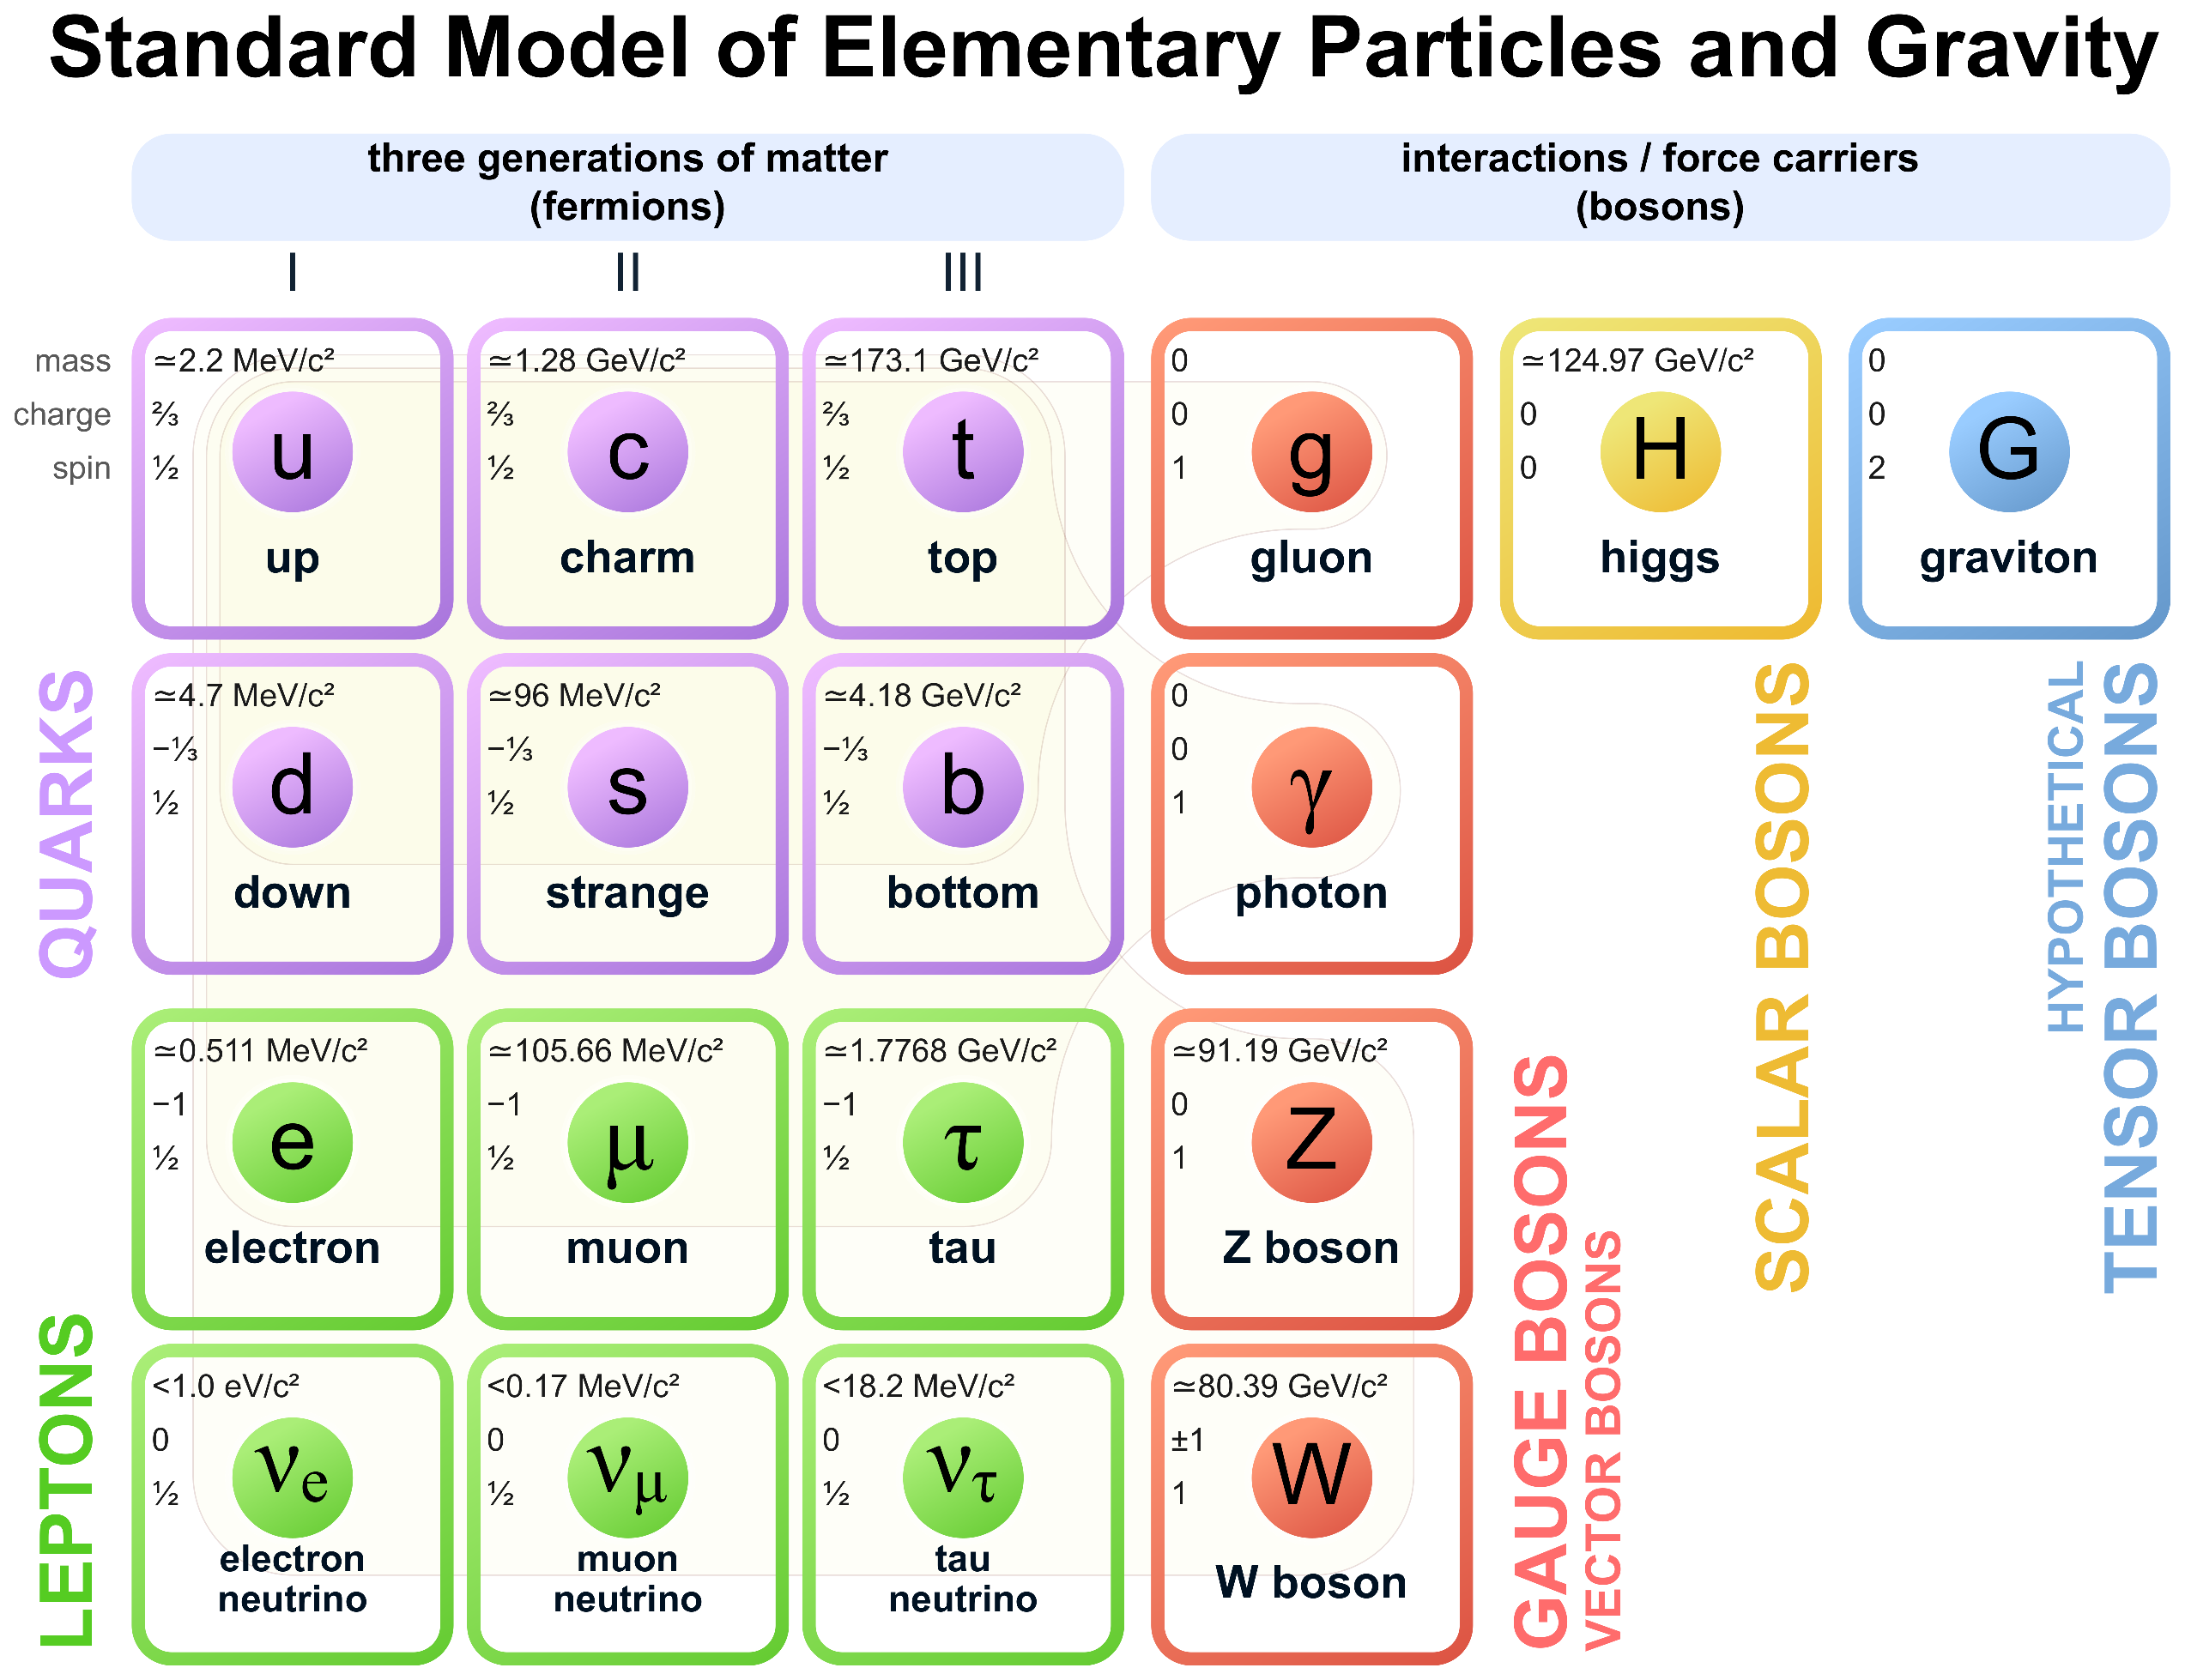
\includegraphics[scale=0.34]{MainContent/Figs/SM.eps}
	\caption{The Standard Model of fundamental particles. Retrieved from}
	\label{fig:sm}
\end{figure}

\section{QCD}
\section{$B^0_s$}
\subsection{$B^0_s \to J/\psi\phi$}
